\documentclass[11pt,a4paper]{article}

% Page layout and geometry
\usepackage[a4paper,margin=1in,headheight=14pt]{geometry}
\usepackage{fancyhdr}

% Font and typography
\usepackage[T1]{fontenc}
\usepackage[utf8]{inputenc}
\usepackage{lmodern}           % Latin Modern fonts for better rendering
\usepackage{microtype}         % Improved typography and spacing
\usepackage{parskip}           % Better paragraph spacing

% Math and symbols
\usepackage{amsmath,amssymb,amsthm}
\usepackage{mathtools}

% Graphics and colors
\usepackage{graphicx}
\usepackage[dvipsnames,table]{xcolor}
\usepackage{tikz}
\usetikzlibrary{shapes,arrows,positioning,calc}

% Tables and lists
\usepackage{booktabs}
\usepackage{tabularx}
\usepackage{enumitem}
\usepackage{multicol}

% Algorithm packages
\usepackage{algorithm}
\usepackage{algpseudocode}

% Code listings
\usepackage{listings}
\usepackage{inconsolata}       % Better monospace font

% Hyperlinks and references
\usepackage[colorlinks=true,linkcolor=NavyBlue,urlcolor=RoyalBlue,citecolor=OliveGreen]{hyperref}
\usepackage[capitalize,nameinlink]{cleveref}

% Header and footer styling
\pagestyle{fancy}
\fancyhf{}
\fancyhead[L]{\small\textsc{$\pi$-Stack Optimizer Documentation}}
\fancyhead[R]{\small\thepage}

\fancyhead[R]{\small\nouppercase{\leftmark}}
\fancyfoot[C]{\small\thepage}
\renewcommand{\headrulewidth}{0.4pt}
\renewcommand{\footrulewidth}{0.4pt}
\renewcommand{\sectionmark}[1]{\markboth{#1}{}}
\renewcommand{\subsectionmark}[1]{\markboth{#1}{}}

% Custom colors for code listings
\definecolor{codebg}{rgb}{0.95,0.95,0.95}
\definecolor{codegreen}{rgb}{0,0.6,0}
\definecolor{codegray}{rgb}{0.5,0.5,0.5}
\definecolor{codepurple}{rgb}{0.58,0,0.82}

% Listings configuration for Python code
\lstdefinestyle{pythonstyle}{
    backgroundcolor=\color{codebg},
    commentstyle=\color{codegreen}\itshape,
    keywordstyle=\color{NavyBlue}\bfseries,
    numberstyle=\tiny\color{codegray},
    stringstyle=\color{codepurple},
    basicstyle=\ttfamily\small,
    breakatwhitespace=false,
    breaklines=true,
    captionpos=b,
    keepspaces=true,
    numbers=left,
    numbersep=8pt,
    showspaces=false,
    showstringspaces=false,
    showtabs=false,
    tabsize=4,
    frame=single,
    rulecolor=\color{gray!30},
    aboveskip=10pt,
    belowskip=10pt
}
\lstset{style=pythonstyle}

% Section styling
\usepackage{titlesec}
\titleformat{\section}
  {\normalfont\Large\bfseries\color{NavyBlue}}{}{0em}{}
\titleformat{\subsection}
  {\normalfont\large\bfseries\color{RoyalBlue}}{}{0em}{}
\titleformat{\subsubsection}
  {\normalfont\normalsize\bfseries\color{MidnightBlue}}{}{0em}{}

% Custom commands
\newcommand{\code}[1]{\texttt{\small #1}}
\newcommand{\file}[1]{\texttt{\textcolor{Maroon}{#1}}}
\newcommand{\func}[1]{\texttt{\textcolor{NavyBlue}{#1}}}
\newcommand{\pkg}[1]{\textsf{#1}}

% Algorithm styling
\algrenewcommand\algorithmicrequire{\textbf{Input:}}
\algrenewcommand\algorithmicensure{\textbf{Output:}}

% Title formatting
\title{%
  \vspace{-1cm}
  {\Huge\bfseries\color{NavyBlue} $\pi$-Stack Optimizer}\\[0.5em]
  {\Large\color{RoyalBlue} User Guide and Technical Documentation}\\[0.3em]
  \rule{\textwidth}{1.5pt}
}
\author{%
  \large Arunima Ghosh, Susmita Barik, Roshan J. Singh and Sandeep K. Reddy\\
  %\small\texttt{Molecular Stacking Optimization Framework}
}
\date{\large Version 1.0 -- \today}

\begin{document}
\maketitle
\thispagestyle{fancy}

\begin{abstract}
\noindent
The \textbf{$\pi$-Stack Optimizer} is a high-performance computational framework for discovering energetically favorable stacking configurations in molecular systems. Leveraging semi-empirical quantum chemistry (xTB) coupled with multiple global optimization algorithms (PSO, GA, GWO, PSO+Nelder-Mead), this tool provides researchers with a flexible, efficient, and reproducible workflow for $\pi$-stacking studies. The system features parallel energy evaluations, automatic symmetry detection, and comprehensive logging capabilities, making it suitable for both exploratory research and production computational chemistry pipelines.
\end{abstract}

\vspace{0.5cm}
\tableofcontents
\newpage

% ============================================================================
% PART 1: INTRODUCTION
% ============================================================================

\section{Introduction}
\label{sec:intro}

\paragraph{Pending note}
{\color{red}Verify SMILES-to-XYZ conversions produce the intended side-chain conformers before dropping monomers into this workflow, because any mistaken geometry is carried through unchanged.}

The $\pi$-Stack Optimizer is a computational tool for finding the most stable arrangements of molecules stacked in one-dimensional columns. When molecules stack together, their relative positions---how far apart they are, how they're rotated, and how they're shifted---determine the stability of the assembly. Finding the best arrangement requires exploring many possible configurations and evaluating their energies, which becomes computationally expensive as the number of possible arrangements grows.

This tool automates the search for optimal stacking configurations by combining quantum chemistry calculations (xTB) with optimization algorithms. Starting from a single monomer structure, the tool systematically explores different stacking arrangements, evaluates their energies, and identifies the most stable configuration. The tool is designed for computational chemists and materials scientists who need to generate realistic starting structures for higher-level calculations, explore how stacking arrangements affect material properties, or study how molecular flexibility influences stacking stability.

The optimization explores a $(7 + N_{\text{torsion}})$-dimensional parameter space that controls how molecules are positioned in the stack:

\begin{equation}
    \mathbf{x} = [c_{\theta}, s_{\theta}, T_x, T_y, T_z, C_x, C_y, \tau_1, \tau_2, \ldots, \tau_{N_{\text{torsion}}}] \in \mathbb{R}^{7+N_{\text{torsion}}}
\end{equation}

The first 7 parameters control the rigid-body transformation (rotation, translation, and rotation center), while the remaining parameters control internal molecular flexibility through dihedral torsions. The optimizer finds parameter values that minimize the binding energy between molecules while avoiding unphysical overlaps.

The tool provides several key capabilities to make this optimization efficient and practical:

\begin{itemize}[leftmargin=2em,itemsep=3pt]
    \item Choose from Particle Swarm Optimization (PSO), Genetic Algorithm (GA), Grey Wolf Optimizer (GWO), or a PSO+Nelder-Mead hybrid, each suited to different problem characteristics.
    
    \item Uses a worker-pool architecture to run multiple quantum chemistry calculations simultaneously, significantly reducing computation time.
    
    \item Supports internal dihedral torsions, allowing flexible parts of molecules to rotate and adapt their shape to optimize stacking interactions.
    
    \item Identifies equivalent torsions in symmetric molecules, reducing the search space and computational cost without losing accuracy.
    
    \item Provides structured console output, trajectory files, and detailed result summaries for analysis and visualization.
    
    \item Clean separation between optimization, geometry handling, and energy evaluation, making it easy to extend or modify components.
\end{itemize}




% ============================================================================
% PART 2: GETTING STARTED
% ============================================================================

\section{Getting Started}
\label{sec:getting-started}

This section will get you up and running with the $\pi$-Stack Optimizer in minutes.


\subsection{Installation}

\subsubsection{Step 1: Clone the Repository}
\begin{lstlisting}[language=bash,style=pythonstyle,numbers=none,frame=single]
git clone https://github.com/sandeepgroup/pi-stack-optimizer.git
cd pi-stack-optimizer
\end{lstlisting}

\subsubsection{Step 2: Create Python Virtual Environment}
\begin{lstlisting}[language=bash,style=pythonstyle,numbers=none,frame=single]
python3 -m venv .venv
source .venv/bin/activate
\end{lstlisting}

\subsubsection{Step 3: Install Python Dependencies}
If a \file{requirements.txt} file is included:
\begin{lstlisting}[language=bash,style=pythonstyle,numbers=none,frame=single]
pip install --upgrade pip
pip install -r requirements.txt
\end{lstlisting}

Otherwise, install \pkg{NumPy} manually:
\begin{lstlisting}[language=bash,style=pythonstyle,numbers=none,frame=single]
pip install numpy
\end{lstlisting}

\subsubsection{Step 4: Enable CLI Wrappers (Recommended)}
Source the helper script to expose the convenience launchers and ensure the repository is on your \texttt{PYTHONPATH}:
\begin{lstlisting}[language=bash,style=pythonstyle,numbers=none,frame=single]
source ./activate_pi_stack.sh
pi-stack-generator --help    # Wrapper for pi-stack-generator.py
pi-hyperopt --help           # Wrapper for hyperparameter-opt/hyperopt.py
\end{lstlisting}
This step sets up shell functions so you can run the tools without typing \code{python path/to/script.py}. If you skip it, prefix the commands with \code{python} and provide the relative script path manually.

\subsubsection{Step 5: Configure xTB Backend}
Verify xTB is accessible:
\begin{lstlisting}[language=bash,style=pythonstyle,numbers=none,frame=single]
which xtb
xtb --version
\end{lstlisting}

Set environment variables if needed:
\begin{lstlisting}[language=bash,style=pythonstyle,numbers=none,frame=single]
export XTBHOME=/path/to/xtb
export OMP_NUM_THREADS=4
\end{lstlisting}

\subsubsection{Step 6: Validate Installation}
\begin{lstlisting}[language=bash,style=pythonstyle,numbers=none,frame=single]
pi-stack-generator example.xyz --workers 1 --optimizer pso \
    --max-iters 1 --swarm-size 4
\end{lstlisting}

If successful, you should see initialization messages and a single optimization iteration. When not using the activation script, replace \code{pi-stack-generator} with \code{python pi-stack-generator.py}.

\subsection{Quick Start: Your First Optimization}

Let's optimize a simple benzene dimer geometry using PSO:

\begin{lstlisting}[language=bash,style=pythonstyle,numbers=none,frame=single]
pi-stack-generator benzene.xyz --optimizer pso --workers 4 \
    --swarm-size 30 --max-iters 100
\end{lstlisting}

This assumes you already sourced \file{activate\_pi\_stack.sh}. Without it, run \code{python pi-stack-generator.py ...} instead.

	extbf{What happens:}
\begin{enumerate}[leftmargin=2em,itemsep=3pt]
    \item The tool reads \file{benzene.xyz} and validates the geometry
    \item Initializes 30 particles with random stacking parameters
    \item Spawns 4 parallel xTB worker processes
    \item Runs 100 PSO iterations (or until convergence)
    \item Outputs optimized geometry to \file{optimized\_monomer\_*.xyz}
    \item Saves full results to \file{optimization\_results.txt}
\end{enumerate}

\textbf{Output files:}
\begin{itemize}[leftmargin=2em,itemsep=3pt]
    \item \file{optimized\_monomer\_*.xyz} -- Best monomer geometry
    \item \file{optimized\_stack\_*.xyz} -- 10-layer demonstration stack
    \item \file{optimization\_results.txt} -- Detailed results with energies and parameters
\end{itemize}

% ============================================================================
% PART 3: BASIC USAGE
% ============================================================================

\section{Basic Usage}
\label{sec:basic-usage}

\subsection{Input File Format}

The primary input is a standard XYZ coordinate file:

\begin{lstlisting}[language=bash,style=pythonstyle,numbers=none,frame=single,caption={Example benzene.xyz file}]
12
Benzene monomer
C    0.000    1.396    0.000
C    1.209    0.698    0.000
C    1.209   -0.698    0.000
C    0.000   -1.396    0.000
C   -1.209   -0.698    0.000
C   -1.209    0.698    0.000
H    0.000    2.479    0.000
H    2.147    1.240    0.000
H    2.147   -1.240    0.000
H    0.000   -2.479    0.000
H   -2.147   -1.240    0.000
H   -2.147    1.240    0.000
\end{lstlisting}

\subsection{Common Workflows}

\subsubsection{Basic Rigid Monomer Optimization}

No torsional flexibility; optimize only translation and rotation:

\begin{lstlisting}[language=bash,style=pythonstyle,numbers=none,frame=single]
python main.py molecule.xyz --optimizer pso \
    --swarm-size 50 --max-iters 200 --workers 8
\end{lstlisting}

\subsubsection{Optimization with Torsional Flexibility}

Provide a \file{torsions.json} file defining rotatable bonds:

\begin{lstlisting}[language=bash,style=pythonstyle,numbers=none,frame=single]
python main.py molecule.xyz --optimizer pso \
    --torsions-file torsions.json \
    --swarm-size 60 --max-iters 300
\end{lstlisting}

Example \file{torsions.json}:
\begin{lstlisting}[style=pythonstyle,numbers=none,frame=single]
{
  "indexing": "0-based",
  "torsions": [
    {
      "name": "phenyl_rotation",
      "atoms": [2, 5, 8, 11],
      "rotate_side": "d"
    }
  ]
}
\end{lstlisting}

\subsubsection{Using Symmetry Detection}

For molecules with symmetric torsions, reduce dimensionality automatically:

\begin{lstlisting}[language=bash,style=pythonstyle,numbers=none,frame=single]
python main.py molecule.xyz \
    --torsions-file torsions.json \
    --enable-symmetric-torsions \
    --symmetric-torsion-tolerance 10.0
\end{lstlisting}

\subsubsection{High-Accuracy Optimization}

Use hybrid PSO+Nelder-Mead for tight convergence:

\begin{lstlisting}[language=bash,style=pythonstyle,numbers=none,frame=single]
python main.py molecule.xyz --optimizer pso-nm \
    --swarm-size 80 --max-iters 400 \
    --hybrid-nm-max-iters 200 --hybrid-nm-tol 1e-6 \
    --workers 16
\end{lstlisting}

\subsubsection{Comparing Multiple Algorithms}

Run the same system with different optimizers:

\begin{lstlisting}[language=bash,style=pythonstyle,numbers=none,frame=single]
# PSO
python main.py mol.xyz --optimizer pso --seed 42

# Genetic Algorithm
python main.py mol.xyz --optimizer ga --seed 42

# Grey Wolf Optimizer
python main.py mol.xyz --optimizer gwo --seed 42

# Hybrid
python main.py mol.xyz --optimizer pso-nm --seed 42
\end{lstlisting}

\subsection{Understanding Output}

\subsubsection{Console Output}

The tool prints structured blocks showing:
\begin{itemize}[leftmargin=2em,itemsep=3pt]
    \item System information (OS, CPU, memory)
    \item Input files and molecular properties
    \item Optimizer configuration
    \item xTB backend settings
    \item Iteration-by-iteration progress
    \item Final results summary
\end{itemize}

\subsubsection{Result Files}

\begin{description}[leftmargin=3cm,style=nextline]
    \item[\file{optimization\_results.txt}] Complete summary including:
    \begin{itemize}[noitemsep]
        \item Best objective value and binding energy
        \item Optimized translation, rotation, and torsion parameters
        \item Execution time and evaluation counts
    \end{itemize}
    
    \item[\file{optimized\_monomer\_*.xyz}] Best monomer geometry in XYZ format
    
    \item[\file{optimized\_stack\_*.xyz}] Multi-layer stack for visualization
    
    \item[\file{pso\_trajectory.csv}] (Optional) Particle trajectories when \code{--print-trajectories} is enabled
\end{description}

\subsection{Tips for Effective Optimization}

\begin{center}
\fcolorbox{NavyBlue}{gray!10}{%
\begin{minipage}{0.92\textwidth}
\vspace{0.2cm}
\textbf{\textcolor{NavyBlue}{Best Practices}}

\begin{itemize}[leftmargin=1.5em,itemsep=5pt]
    \item \textbf{Start Small:} Test with \code{--max-iters 10} and small swarm/population to verify setup
    
    \item \textbf{Validate xTB:} Always run \code{xtb --version} before long optimizations
    
    \item \textbf{Match Workers to Cores:} Set \code{--workers} equal to available CPU cores
    
    \item \textbf{Use Trajectory Logging:} Enable \code{--print-trajectories} to diagnose convergence issues
    
    \item \textbf{Set Seeds:} Use \code{--seed} for reproducible results across runs
    
    \item \textbf{Monitor Convergence:} Check \file{optimization\_results.txt} after each run
\end{itemize}
\vspace{0.2cm}
\end{minipage}
}
\end{center}

% ============================================================================
% PART 4: COMMAND-LINE REFERENCE
% ============================================================================

\section{Command-Line Reference}
\label{sec:cli-reference}

This section provides a complete reference for all command-line options.

\subsection{Synopsis}

\begin{lstlisting}[language=bash,style=pythonstyle,numbers=none,frame=single]
python main.py XYZ_FILE [OPTIONS]
\end{lstlisting}

\subsection{Required Arguments}

\begin{description}[leftmargin=3cm,style=nextline]
    \item[\code{XYZ\_FILE}] Path to monomer XYZ coordinate file (\textit{required positional argument})
\end{description}

\subsection{General Options}

\begin{description}[leftmargin=3cm,style=nextline]
    \item[\code{--n-layer}] Number of layers for energy evaluation stack (default: \code{2})
    \item[\code{--optimizer}] Optimization method: \code{pso}, \code{ga}, \code{gwo}, or \code{pso-nm} (default: \code{pso})
    \item[\code{--max-iters}] Maximum optimizer iterations/generations (default: \code{300})
    \item[\code{--seed}] Random seed for reproducible initialization (default: \code{42})
    \item[\code{--verbose-every}] Print progress every N iterations (default: \code{1})
\end{description}

\subsection{xTB Backend Options}

\begin{description}[leftmargin=3cm,style=nextline]
    \item[\code{--workers}] Number of parallel xTB worker processes (default: \code{4})
    \item[\code{--threads}] OpenMP threads per xTB calculation (default: \code{1})
    \item[\code{--method}] xTB method: \code{gfn2}, \code{gfn1}, \code{gfn0}, or \code{gfnff} (default: \code{gfn2})
    \item[\code{--charge}] Total molecular charge (default: \code{0})
    \item[\code{--mult}] Spin multiplicity (default: \code{1})
\end{description}

\subsection{Torsion and Symmetry Options}

\begin{description}[leftmargin=3cm,style=nextline]
    \item[\code{--torsions-file}] Path to JSON file defining dihedral torsions (default: disabled)
    \item[\code{--enable-symmetric-torsions}] Enable automatic symmetry detection (default: disabled)
    \item[\code{--symmetric-torsion-tolerance}] Symmetry tolerance in degrees (default: \code{10.0}°)
\end{description}

\subsection{Penalty Function Options}

\begin{description}[leftmargin=3cm,style=nextline]
    \item[\code{--penalty-weight}] Clash penalty weight (default: \code{2.0})
    \item[\code{--clash-cutoff}] Clash detection cutoff in Ångströms (default: \code{1.6} Å)
    \item[\code{--intramol-penalty-weight}] Intramolecular clash penalty weight (default: \code{5.0})
    \item[\code{--intramol-cutoff}] Intramolecular clash cutoff in Ångströms (default: \code{1.2} Å)
\end{description}

\subsection{PSO-Specific Options}

\begin{description}[leftmargin=3cm,style=nextline]
    \item[\code{--swarm-size}] Number of particles in swarm (default: \code{60})
    \item[\code{--inertia}] Inertia weight (default: \code{0.73})
    \item[\code{--cognitive}] Cognitive coefficient (default: \code{1.50})
    \item[\code{--social}] Social coefficient (default: \code{1.50})
    \item[\code{--tol}] Convergence tolerance for early stopping (default: \code{0.01})
    \item[\code{--patience}] Iterations to wait before early stopping (default: \code{20})
    \item[\code{--print-trajectories}] Enable CSV trajectory logging (default: \code{False})
\end{description}

\subsection{Genetic Algorithm Options}

\begin{description}[leftmargin=3cm,style=nextline]
    \item[\code{--ga-population}] Population size (default: \code{80})
    \item[\code{--ga-elite-fraction}] Elite fraction (default: \code{0.10})
    \item[\code{--ga-tournament-size}] Tournament size (default: \code{3})
    \item[\code{--ga-crossover-rate}] Crossover probability (default: \code{0.90})
    \item[\code{--ga-mutation-rate}] Mutation probability (default: \code{0.10})
    \item[\code{--ga-mutation-sigma}] Mutation noise standard deviation (default: \code{0.30})
    \item[\code{--ga-tol}] Convergence tolerance for early stopping (default: \code{0.01})
    \item[\code{--ga-patience}] Generations to wait before early stopping (default: \code{20})
\end{description}

\subsection{Grey Wolf Optimizer Options}

\begin{description}[leftmargin=3cm,style=nextline]
    \item[\code{--gwo-pack-size}] Number of wolves (default: \code{50})
    \item[\code{--gwo-a-start}] Initial exploration parameter (default: \code{2.0})
    \item[\code{--gwo-a-end}] Final exploration parameter (default: \code{0.0})
    \item[\code{--gwo-tol}] Convergence tolerance for early stopping (default: \code{0.01})
    \item[\code{--gwo-patience}] Iterations to wait before early stopping (default: \code{20})
\end{description}

\subsection{PSO+Nelder-Mead Hybrid Options}

\begin{description}[leftmargin=3cm,style=nextline]
    \item[\code{--hybrid-nm-max-iters}] Maximum NM iterations (default: \code{200})
    \item[\code{--hybrid-nm-initial-step}] Initial simplex step size (default: \code{0.20})
    \item[\code{--hybrid-nm-alpha}] Reflection coefficient (default: \code{1.0})
    \item[\code{--hybrid-nm-gamma}] Expansion coefficient (default: \code{2.0})
    \item[\code{--hybrid-nm-rho}] Contraction coefficient (default: \code{0.50})
    \item[\code{--hybrid-nm-sigma}] Shrink coefficient (default: \code{0.50})
    \item[\code{--hybrid-nm-tol}] Convergence tolerance (default: \code{0.01})
\end{description}

\subsection{Getting Help}

\begin{lstlisting}[language=bash,style=pythonstyle,numbers=none,frame=single]
pi-stack-generator --help
\end{lstlisting}
Use \code{python pi-stack-generator.py --help} if you have not sourced the activation script.

% ============================================================================
% PART 5: WORKFLOW OVERVIEW
% ============================================================================

\section{Workflow Overview}
\label{sec:workflow-overview}

Before diving into implementation details, this section provides a high-level view of how the $\pi$-Stack Optimizer processes molecular inputs to discover optimal stacking configurations.

\subsection{Conceptual Pipeline}

The optimization workflow follows a clear data transformation pipeline from molecular input to optimized stack geometries:

\begin{figure}[H]
\centering
\resizebox{\textwidth}{!}{%
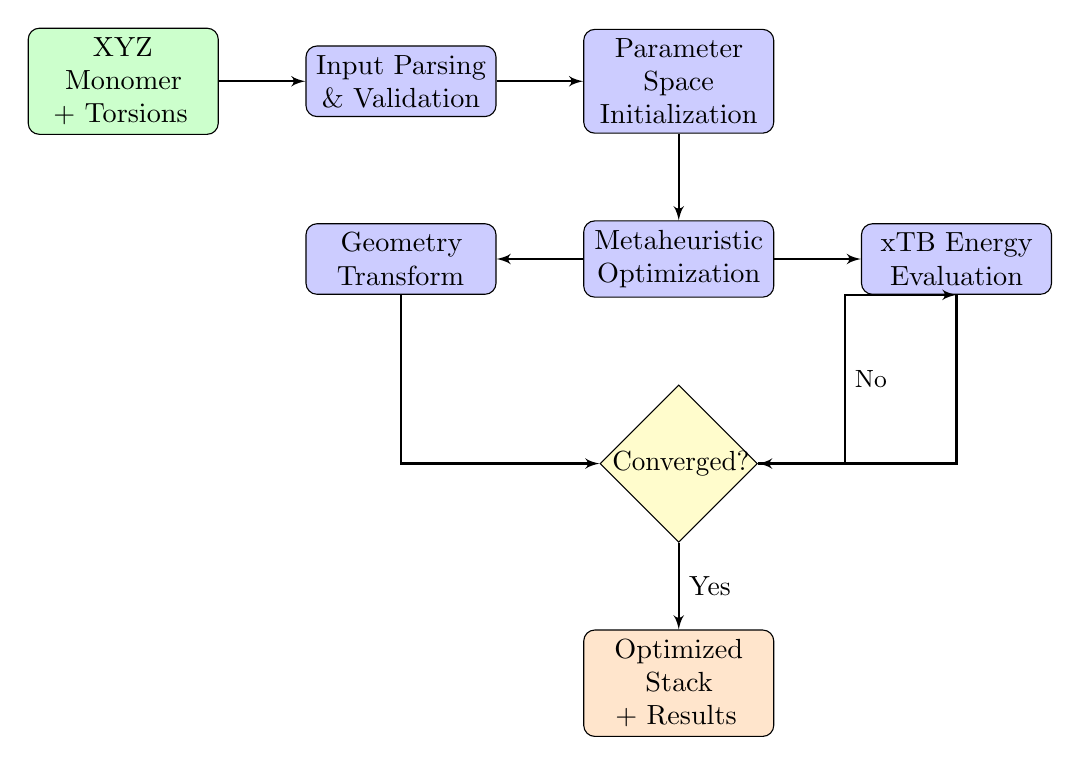
\begin{tikzpicture}[node distance=1.1cm, auto,
    input/.style={rectangle, draw, fill=green!20, text width=6.2em, text centered, rounded corners, minimum height=2em},
    process/.style={rectangle, draw, fill=blue!20, text width=6.2em, text centered, rounded corners, minimum height=2em},
    output/.style={rectangle, draw, fill=orange!20, text width=6.2em, text centered, rounded corners, minimum height=2em},
    decision/.style={diamond, draw, fill=yellow!20, text width=4.8em, text badly centered, inner sep=0pt, minimum height=2em},
    line/.style={draw, -latex', thick}]
    
    % Top row - Input and initial processing
    \node [input] (xyz) {XYZ Monomer\\+ Torsions};
    \node [process, right=of xyz] (parse) {Input Parsing\\\& Validation};
    \node [process, right=of parse] (init) {Parameter Space\\Initialization};
    
    % Middle row - Optimization loop
    \node [process, below=of init] (optim) {Metaheuristic\\Optimization};
    \node [process, left=of optim] (transform) {Geometry\\Transform};
    \node [process, right=of optim] (evaluate) {xTB Energy\\Evaluation};
    
    % Bottom row - Decision and output
    \node [decision, below=of optim] (converge) {Converged?};
    \node [output, below=of converge] (results) {Optimized Stack\\+ Results};
    
    % Flow connections
    \path [line] (xyz) -- (parse);
    \path [line] (parse) -- (init);
    \path [line] (init) -- (optim);
    \path [line] (optim) -- (transform);
    \path [line] (optim) -- (evaluate);
    \path [line] (transform) |- (converge);
    \path [line] (evaluate) |- (converge);
    \path [line] (converge) -- node {Yes} (results);
    \path [line] (converge.east) -| ++(1.1,0) |- (evaluate.south) node [near start, right, font=\small] {No};
\end{tikzpicture}
}
\caption{High-level workflow showing the iterative optimization loop between parameter updates and energy evaluations.}
\label{fig:workflow-overview}
\end{figure}

The workflow transforms a single monomer structure into an optimized supramolecular assembly through iterative refinement:

\begin{center}
\fcolorbox{NavyBlue}{gray!5}{%
\begin{minipage}{0.9\textwidth}
\vspace{0.3cm}
\textbf{Input:} Monomer XYZ + Optional Torsions\\[0.2cm]
$\downarrow$ \textit{Parameter space definition}\\[0.2cm]
\textbf{Search:} $\mathbf{x} = [c_{\theta}, s_{\theta}, T_x, T_y, T_z, C_x, C_y, \tau_1, \ldots, \tau_n]$\\[0.2cm]
$\downarrow$ \textit{Geometry construction + Energy evaluation}\\[0.2cm]
\textbf{Objective:} $f(\mathbf{x}) = E_{\text{bind}} + \text{Clash Penalties}$\\[0.2cm]
$\downarrow$ \textit{Metaheuristic optimization}\\[0.2cm]
\textbf{Output:} Optimized Stack + Analysis
\vspace{0.3cm}
\end{minipage}
}
\end{center}

This modular design ensures that new optimization algorithms, energy methods, or geometric constraints can be integrated with minimal code changes, making the framework suitable for both routine screening and methodological research.

% ============================================================================
% PART 6: TECHNICAL DETAILS
% ============================================================================

\section{Technical Details}
\label{sec:technical-details}

\subsection{Software Architecture}

The system follows a modular pipeline architecture with clear separation of concerns:

\begin{figure}[h]
\centering
\begin{tabular}{c}
\texttt{pi-stack-generator.py} \\
$\downarrow$ \\
\texttt{modules/xyz\_io.py} \\
$\downarrow$ \\
\texttt{modules/geometry.py} \\
$\downarrow$ \\
\texttt{modules/objective.py} $\rightarrow$ \texttt{modules/xtb\_workers.py} \\
$\downarrow$ \\
\texttt{modules/optimizer.py} \\
$\downarrow$ \\
\texttt{modules/reporting.py}
\end{tabular}
\caption{High-level workflow pipeline showing data flow through core modules.}
\label{fig:architecture}
\end{figure}

\subsubsection{Module Responsibilities}

\begin{description}[leftmargin=3cm,style=nextline]
    \item[\file{pi-stack-generator.py}] Orchestrates workflow, parses CLI, initializes components, manages output
    
    \item[\file{modules/xyz\_io.py}] Validates XYZ files, reads/writes molecular coordinates
    
    \item[\file{modules/geometry.py}] Handles coordinate transformations, torsion application, clash detection
    
    \item[\file{modules/objective.py}] Defines objective function interface, implements batch evaluation
    
    \item[\file{modules/xtb\_workers.py}] Manages parallel xTB processes, handles scratch directories, implements performance optimizations
    
    \item[\file{modules/optimizer.py}] Factory pattern for algorithm selection, implements PSO/GA/GWO/Hybrid
    
    \item[\file{modules/reporting.py}] Generates result summaries and parameter formatting
\end{description}

\subsection{Computational Workflow}

\subsubsection{Parameter Space Definition}

The optimization explores a $(7 + N_{\text{torsion}})$-dimensional space consisting of 7 rigid-body transformation parameters and $N_{\text{torsion}}$ internal dihedral angles:

\begin{equation}
    \mathbf{x} = [c_{\theta}, s_{\theta}, T_x, T_y, T_z, C_x, C_y, \tau_1, \tau_2, \ldots, \tau_{N_{\text{torsion}}}] \in \mathbb{R}^{7+N_{\text{torsion}}}
\end{equation}

where the first 7 parameters define a rotation-around-center transformation.

\paragraph{Seven-Dimensional Transformation Parameterization}

Instead of using Euler angles (which suffer from gimbal lock and discontinuities), the code employs a rotation-around-center parameterization with 7 parameters:

\begin{itemize}[leftmargin=2em,itemsep=2pt]
    \item $c_{\theta}, s_{\theta}$: Trigonometric components encoding rotation angle $\theta$ (dimensionless)
    \item $T_x, T_y, T_z$: Translation vector components (Ångströms)
    \item $C_x, C_y$: Center-of-rotation coordinates in the $xy$-plane (Ångströms)
\end{itemize}

\paragraph{Transformation Matrix}

The transformation combines rotation around an arbitrary center $(C_x, C_y, 0)$ with translation. We derive the transformation matrix step by step, starting from basic geometric operations.

\subparagraph{Step 1: Rotation Angle Recovery}

The optimization parameters $c_{\theta}$ and $s_{\theta}$ encode the rotation angle without $2\pi$ periodicity issues. The actual rotation angle $\theta$ is recovered as:
\begin{equation}
    \theta = \arctan2(s_{\theta}, c_{\theta})
    \label{eq:angle-recovery}
\end{equation}

From this angle, we compute the standard trigonometric values:
\begin{equation}
    c = \cos\theta, \qquad s = \sin\theta
    \label{eq:trig-values}
\end{equation}

\subparagraph{Step 2: Rotation Around Origin}

A rotation by angle $\theta$ around the $z$-axis (origin) transforms a point $(x, y, z)$ to:
\begin{equation}
    \begin{bmatrix} x' \\ y' \\ z' \end{bmatrix} = \begin{bmatrix}
        c & -s & 0 \\
        s &  c & 0 \\
        0 &  0 & 1
    \end{bmatrix} \begin{bmatrix} x \\ y \\ z \end{bmatrix}
    = \begin{bmatrix}
        cx - sy \\
        sx + cy \\
        z
    \end{bmatrix}
    \label{eq:rotation-origin}
\end{equation}

\subparagraph{Step 3: Rotation Around Arbitrary Center}

To rotate around an arbitrary center $\mathbf{C} = (C_x, C_y, 0)$ instead of the origin, we:
\begin{enumerate}[leftmargin=2em,itemsep=2pt]
    \item Translate by $-\mathbf{C}$ to move the center to the origin
    \item Apply the rotation around the origin
    \item Translate back by $+\mathbf{C}$
\end{enumerate}

This yields the transformation:
\begin{equation}
    \mathbf{p}' = \mathbf{R}(\theta) (\mathbf{p} - \mathbf{C}) + \mathbf{C} = \mathbf{R}(\theta) \mathbf{p} + (\mathbf{C} - \mathbf{R}(\theta) \mathbf{C})
    \label{eq:rotation-center}
\end{equation}

where $\mathbf{R}(\theta)$ is the rotation matrix from \cref{eq:rotation-origin}. Expanding the center correction term:
\begin{align}
    \mathbf{C} - \mathbf{R}(\theta) \mathbf{C} &= \begin{bmatrix} C_x \\ C_y \\ 0 \end{bmatrix} - \begin{bmatrix}
        c & -s & 0 \\
        s &  c & 0 \\
        0 &  0 & 1
    \end{bmatrix} \begin{bmatrix} C_x \\ C_y \\ 0 \end{bmatrix} \nonumber\\
    &= \begin{bmatrix} C_x \\ C_y \\ 0 \end{bmatrix} - \begin{bmatrix}
        c C_x - s C_y \\
        s C_x + c C_y \\
        0
    \end{bmatrix} \nonumber\\
    &= \begin{bmatrix}
        C_x - (c C_x - s C_y) \\
        C_y - (s C_x + c C_y) \\
        0
    \end{bmatrix}
    \label{eq:center-correction}
\end{align}

\subparagraph{Step 4: Adding Translation}

The optimization parameters include an additional translation vector $\mathbf{T} = (T_x, T_y, T_z)$. The complete transformation becomes:
\begin{equation}
    \mathbf{p}' = \mathbf{R}(\theta) \mathbf{p} + (\mathbf{C} - \mathbf{R}(\theta) \mathbf{C}) + \mathbf{T}
    \label{eq:full-transform}
\end{equation}

Combining the center correction and translation terms, we obtain the effective displacement vector:
\begin{align}
    d_x &= T_x + C_x - (c C_x - s C_y) = T_x + C_x - c C_x + s C_y \nonumber\\
    d_y &= T_y + C_y - (s C_x + c C_y) = T_y + C_y - s C_x - c C_y \nonumber\\
    d_z &= T_z
    \label{eq:displacement-vector}
\end{align}

\subparagraph{Step 5: Homogeneous Transformation Matrix}

Expressing the transformation in homogeneous coordinates (4D) allows us to represent both rotation and translation as a single matrix multiplication. The final $4 \times 4$ transformation matrix is:
\begin{equation}
    \mathbf{M} = \begin{bmatrix}
        c & -s & 0 & d_x \\
        s &  c & 0 & d_y \\
        0 &  0 & 1 & T_z \\
        0 &  0 & 0 & 1
    \end{bmatrix}
    \label{eq:transformation-matrix-final}
\end{equation}

where $c = \cos\theta$ and $s = \sin\theta$ are computed from the optimization parameters via \cref{eq:angle-recovery} and \cref{eq:trig-values}, and $d_x, d_y$ are given by \cref{eq:displacement-vector}.

\subparagraph{Step 6: Coordinate Transformation}

For a coordinate $\mathbf{p} = (x, y, z)^T$, the transformed coordinate in homogeneous form is:
\begin{equation}
    \begin{bmatrix} x' \\ y' \\ z' \\ 1 \end{bmatrix} = \mathbf{M} \begin{bmatrix} x \\ y \\ z \\ 1 \end{bmatrix}
    = \begin{bmatrix}
        c & -s & 0 & d_x \\
        s &  c & 0 & d_y \\
        0 &  0 & 1 & T_z \\
        0 &  0 & 0 & 1
    \end{bmatrix} \begin{bmatrix} x \\ y \\ z \\ 1 \end{bmatrix}
    = \begin{bmatrix}
        cx - sy + d_x \\
        sx + cy + d_y \\
        z + T_z \\
        1
    \end{bmatrix}
    \label{eq:coordinate-transform}
\end{equation}

The final 3D coordinates are obtained by extracting the first three components: $\mathbf{p}' = (x', y', z')^T$.

\paragraph{Multi-Layer Stack Construction}

For an $N$-layer stack, successive layers are generated by repeated application of $\mathbf{M}$:
\begin{equation}
    \text{Layer } k: \quad \mathbf{p}_k = \mathbf{M}^k \mathbf{p}_0, \quad k = 0, 1, 2, \ldots, N-1
    \label{eq:stack-construction}
\end{equation}

where $\mathbf{p}_0$ is the base monomer coordinate and $\mathbf{M}^k = \underbrace{\mathbf{M} \cdot \mathbf{M} \cdots \mathbf{M}}_{k \text{ times}}$ is the $k$-th matrix power.

\paragraph{Optimization Bounds}

The parameter space is initialized with Gaussian distributions centered at reasonable physical values:

\begin{table}[H]
\centering
\begin{tabular}{lcc}
\toprule
\textbf{Parameter} & \textbf{Initialization} & \textbf{Physical Meaning} \\
\midrule
$c_{\theta}$ & $\mathcal{N}(0, 1)$ & Cosine-like component (unbounded) \\
$s_{\theta}$ & $\mathcal{N}(0, 1)$ & Sine-like component (unbounded) \\
$T_x$ & $\mathcal{N}(0, 2.0)$ Å & $x$-translation \\
$T_y$ & $\mathcal{N}(0, 2.0)$ Å & $y$-translation \\
$T_z$ & $\mathcal{N}(3.5, 1.0)$ Å & $z$-translation (typical $\pi$-stacking distance) \\
$C_x$ & $\mathcal{N}(0, 2.0)$ Å & Rotation center $x$-coordinate \\
$C_y$ & $\mathcal{N}(0, 2.0)$ Å & Rotation center $y$-coordinate \\
$\tau_i$ & $\mathcal{N}(0, 0.5)$ rad & Torsion angle $i$, clipped to $[-\pi, \pi]$ \\
\bottomrule
\end{tabular}
\caption{Parameter initialization distributions for swarm-based optimizers.}
\label{tab:param-bounds}
\end{table}

\textbf{Rationale:}
\begin{itemize}[leftmargin=2em,itemsep=2pt]
    \item Using $(c_{\theta}, s_{\theta})$ instead of $\theta$ directly avoids $2\pi$ periodicity and allows continuous exploration
    \item $T_z \sim \mathcal{N}(3.5, 1.0)$ centers the search around typical $\pi$-stacking distances (3–4 Å)
    \item In-plane parameters $(T_x, T_y, C_x, C_y)$ use wider distributions to explore lateral shifts and rotation centers
    \item Torsion angles are clipped to $[-\pi, \pi]$ to maintain physical relevance
\end{itemize}

\paragraph{Parameter Bounds and Clamping}

To prevent the optimizer from exploring unphysical regions of parameter space, all optimization algorithms enforce hard bounds on parameters after each update step. These bounds are critical for preventing optimizer drift (particularly in PSO) that can lead to extreme parameter values and xTB calculation failures.

\begin{table}[H]
\centering
\begin{tabular}{lcc}
\toprule
\textbf{Parameter} & \textbf{Lower Bound} & \textbf{Upper Bound} \\
\midrule
$c_{\theta}$ & $-1.0$ & $+1.0$ \\
$s_{\theta}$ & $-1.0$ & $+1.0$ \\
$T_x$ & $-10.0$ Å & $+10.0$ Å \\
$T_y$ & $-10.0$ Å & $+10.0$ Å \\
$T_z$ & $+2.0$ Å & $+6.0$ Å \\
$C_x$ & $-10.0$ Å & $+10.0$ Å \\
$C_y$ & $-10.0$ Å & $+10.0$ Å \\
$\tau_i$ & $-2\pi$ rad & $+2\pi$ rad \\
\bottomrule
\end{tabular}
\caption{Hard parameter bounds enforced after each optimizer update. Parameters are clamped to these ranges using \code{np.clip}.}
\label{tab:param-bounds-enforcement}
\end{table}

\textbf{Implementation:} After each position update in PSO (and similarly for other algorithms), the \func{\_clamp\_positions} function applies:
\begin{equation}
    x_i \leftarrow \text{clip}(x_i, x_{i,\min}, x_{i,\max})
\end{equation}
This prevents accumulation of unrealistic values that could arise from unbounded velocity updates in PSO or mutation/crossover operations in GA. The bounds are defined in \code{PARAM\_BOUNDS} dictionary in \file{modules/optimizer.py}.

\subsubsection{Objective Function Evaluation}

\paragraph{Evaluation Pipeline}

For each candidate vector $\mathbf{x} \in \mathbb{R}^{7+N_{\text{torsion}}}$ the optimizer executes a fixed series of transformations:

\begin{description}[leftmargin=2.5em,style=nextline,itemsep=2pt]
    \item[Parameter extraction] Partition $\mathbf{x}$ into rigid-body parameters $\mathbf{x}_{\text{rigid}} \in \mathbb{R}^7$ and torsions $\boldsymbol{\tau} \in \mathbb{R}^{N_{\text{torsion}}}$.
    \item[Torsion application] Apply each torsion in $\boldsymbol{\tau}$ to the relevant fragment, producing the modified monomer coordinates $\mathbf{p}_{\text{mono}}$.
    \item[Stack construction] Build the transformation matrix $\mathbf{M}$ from $\mathbf{x}_{\text{rigid}}$ and replicate the monomer by powers of $\mathbf{M}$ to obtain the $N$-layer stack.
    \item[Clash analysis] Evaluate inter-layer and intra-molecular overlaps to obtain preliminary penalty terms $P_{\text{inter}}$ and $P_{\text{intra}}$ (detailed below).
    \item[Energy sampling] Dispatch both the relaxed monomer and the stacked geometry to the xTB worker pool to retrieve $E_{\text{mono}}$ and $E_{\text{stack}}$.
\end{description}

\paragraph{Energy Component}

The physics-based portion of the objective is the per-interface binding energy:
\begin{equation}
    E_{\text{bind}} = \frac{E_{\text{stack}} - N \cdot E_{\text{mono}}}{N - 1} \times 2625.5 \quad \text{(kJ/mol)}
    \label{eq:binding-energy}
\end{equation}
which converts Hartree differences to kJ/mol and normalizes by the number of interfaces to make systems with different $N$ directly comparable.

\paragraph{Clash Penalty Models}

Clash penalties prevent unphysical geometries where atoms approach closer than van der Waals radii. Two complementary models are applied:

\textbf{Inter-layer penalty ($P_{\text{inter}}$):} Captures overlaps between distinct layers in the stack with cutoff $r_{\text{inter}} = 1.6$ Å. The penalty uses geometric weights $w_{ij} = \frac{1}{j-i}$ so closer layers carry higher penalties.

\textbf{Intra-molecular penalty ($P_{\text{intra}}$):} Suppresses clashes inside the monomer caused by torsion rotations, with cutoff $r_{\text{intra}} = 1.2$ Å. The exclusion list removes bonded (1-2) and angle (1-3) pairs, ensuring only non-bonded contacts contribute.

\paragraph{Combined Objective and Failure Handling}

Binding energy alone cannot guarantee chemically valid structures, so the optimizer augments it with the clash models above. The first step is to accumulate a single scalar penalty:

\begin{equation}
    P_{\text{total}} = P_{\text{inter}} + w_{\text{intra}} \cdot P_{\text{intra}}
    \label{eq:total-penalty}
\end{equation}

where $w_{\text{intra}} = 5.0$ is the intra-molecular penalty weight. For successful xTB evaluations, the fitness is:
\begin{equation}
    f(\mathbf{x}) = E_{\text{bind}} + c_{\text{clash}} \cdot P_{\text{total}}
    \label{eq:objective-success}
\end{equation}
where $E_{\text{bind}}$ is the per-interface binding energy in kJ/mol and $c_{\text{clash}} = 10{,}000$ ensures clash penalties dominate when present.

Failed xTB calculations (e.g., SCF divergence caused by extreme clashes) receive a shifted objective

\begin{equation}
    f_{\text{fail}}(\mathbf{x}) = c_{\text{base}} + c_{\text{clash}} \cdot P_{\text{total}}
    \label{eq:objective-failure}
\end{equation}

with $c_{\text{base}} = 1{,}000{,}000$ (FAILURE\_PENALTY\_BASE). The additive $c_{\text{clash}} P_{\text{total}}$ term still differentiates degrees of failure, nudging the search toward less pathological geometries before re-entering the feasible region.

\paragraph{Penalty Summary}

\begin{table}[H]
\centering
\begin{tabular}{lcl}
\toprule
\textbf{Parameter} & \textbf{Value} & \textbf{Purpose} \\
\midrule
$w_{\text{intra}}$ & 5.0 & Weight for intra-molecular penalties in $P_{\text{total}}$ \\
$c_{\text{clash}}$ & 10{,}000 & Clash penalty multiplier (FAILURE\_PENALTY\_CLASH\_MULT) \\
$c_{\text{base}}$ & 1{,}000{,}000 & Base penalty for failed calculations (FAILURE\_PENALTY\_BASE) \\
$r_{\text{inter}}$ & 1.6 Å & Inter-molecular clash cutoff distance \\
$r_{\text{intra}}$ & 1.2 Å & Intra-molecular clash cutoff distance \\
\bottomrule
\end{tabular}
\caption{Clash penalty constants and their roles in the objective function.}
\label{tab:penalty-parameters}
\end{table}

\paragraph{Behavior Across Regimes}

Because $c_{\text{base}} \gg c_{\text{clash}} \gg |E_{\text{bind}}|$, the fitness landscape separates into three intuitive bands:
\begin{itemize}[leftmargin=2em,itemsep=2pt]
    \item \textbf{Failed geometries ($f > 10^6$):} Always worse than any converged point but still ranked by clash magnitude to steer the search toward milder failures.
    \item \textbf{Clash-prone geometries ($50 < f < 10^6$):} Dominated by $c_{\text{clash}} P_{\text{total}}$, forcing rapid movement toward feasible regions.
    \item \textbf{Valid geometries ($-50 < f < 50$):} Essentially clash-free so the optimizer compares solutions purely on binding energy.
\end{itemize}

\subsubsection{xTB Parallel Execution}

The xTB quantum chemistry calculations are parallelized using a worker pool architecture to maximize computational throughput. The implementation leverages Python's \pkg{multiprocessing.Pool} to spawn independent worker processes, each maintaining an isolated scratch directory for file I/O operations. The system uses only command-line xTB binaries (no tblite dependency) and includes several performance optimizations.

\paragraph{Worker Pool Architecture}

The parallel execution workflow proceeds as follows:

\begin{itemize}[leftmargin=2em,itemsep=3pt]
    \item At program startup, spawn $N_{\text{workers}}$ independent processes. Each worker creates an isolated temporary directory to avoid file conflicts and remains idle, waiting for geometry submission requests.
    
    \item The main optimization loop submits batches of molecular geometries to the worker pool queue. Each submission includes atom types, Cartesian coordinates, and a unique job identifier. Jobs are distributed to available workers using a FIFO scheduling policy.
    
    \item Each worker receives a geometry, writes it to an XYZ file in its scratch directory, invokes the xTB binary with command \code{xtb --gfn2 --sp} for single-point GFN2-xTB energy calculation, and parses the output file to extract the total energy in Hartrees.
    
    \item Computed energies are returned to the main process via a result queue, where they are matched to their originating job IDs. If xTB reports an error (e.g., SCF convergence failure), the worker returns an error flag instead of an energy value.
    
    \item Upon optimization completion, all worker processes are terminated gracefully, and their temporary directories are recursively removed to avoid accumulating scratch files on disk.
\end{itemize}

\paragraph{Performance Considerations}

The number of workers $N_{\text{workers}}$ should be chosen based on available CPU cores and xTB's threading behavior. Each xTB worker internally uses OpenMP threads (controlled by \code{OMP\_NUM\_THREADS}), so the total thread count is approximately:
\begin{equation}
    N_{\text{threads,total}} \approx N_{\text{workers}} \times N_{\text{OMP}}
    \label{eq:thread-scaling}
\end{equation}

For optimal performance on a machine with $N_{\text{CPU}}$ cores, typical configurations are:
\begin{itemize}[leftmargin=2em,itemsep=2pt]
    \item \textbf{High parallelism:} $N_{\text{workers}} = N_{\text{CPU}}$, $N_{\text{OMP}} = 1$ (many small jobs, minimal inter-thread synchronization overhead)
    \item \textbf{Balanced:} $N_{\text{workers}} = N_{\text{CPU}}/4$, $N_{\text{OMP}} = 4$ (moderate parallelism with some threading efficiency)
    \item \textbf{Low parallelism:} $N_{\text{workers}} = N_{\text{CPU}}/8$, $N_{\text{OMP}} = 8$ (few large jobs, higher per-job threading efficiency)
\end{itemize}

\subsection{Symmetry Detection}

Molecular symmetry can drastically reduce the search dimensionality by identifying torsion angles that should remain equivalent due to chemical equivalence. When the \code{--enable-symmetric-torsions} flag is activated, the optimizer applies an automated symmetry detection algorithm.

\paragraph{Symmetry Detection Algorithm}

The algorithm identifies groups of torsions that are chemically equivalent by analyzing local bonding environments:

\begin{table}[H]
\centering
\begin{tabular}{cp{11cm}}
\toprule
\textbf{Step} & \textbf{Procedure} \\
\midrule
1 & \textbf{Pairwise Comparison:} For each pair of torsion definitions $(T_i, T_j)$, compare the four defining atoms and their immediate bonding neighborhoods to detect structural similarity. \\[0.5em]
2 & \textbf{Environment Matching:} Two torsions are considered equivalent if their central bond atoms have identical element types and bond orders, and their peripheral atoms (defining the dihedral) have matching connectivity patterns within a specified tolerance. \\[0.5em]
3 & \textbf{Grouping:} Cluster all mutually equivalent torsions into symmetry groups. Each group $\mathcal{G}_k = \{T_{k,1}, T_{k,2}, \ldots, T_{k,m_k}\}$ contains $m_k$ symmetric torsions that will share a single control parameter. \\[0.5em]
4 & \textbf{Dimension Reduction:} Map the original $N_{\text{torsion}}$ independent torsion angles to $N_{\text{reduced}} = |\{\mathcal{G}_k\}|$ control variables. The dimensionality reduction factor is $\Delta = N_{\text{torsion}} - N_{\text{reduced}}$. \\[0.5em]
5 & \textbf{Expansion:} During objective function evaluation, expand the reduced parameter vector by applying the same angle to all torsions in each symmetry group, ensuring physical consistency. \\
\bottomrule
\end{tabular}
\caption{Five-step symmetry detection and dimension reduction algorithm.}
\label{tab:symmetry-algorithm}
\end{table}

\paragraph{Impact on Optimization Efficiency}

Symmetry detection provides substantial benefits for molecules with repeated structural motifs. Consider a benzene derivative with six equivalent methyl rotors: without symmetry detection, the optimizer explores a $(7 + 6) = 13$-dimensional space; with symmetry detection, this reduces to $(7 + 1) = 8$ dimensions, decreasing computational cost by approximately $\left(\frac{13}{8}\right)^2 \approx 2.6\times$ for swarm-based methods where cost scales roughly as $\mathcal{O}(d^2)$.

The symmetry tolerance parameter (default: $10^{-3}$ Å for distance comparisons) controls the strictness of environment matching. Tighter tolerances reduce false positives but may miss genuine symmetries in slightly distorted geometries.

\subsection{Logging and Output}

\subsubsection{Console Output Structure}

Structured ASCII blocks always appear in the same order. A banner opens the run and shows authors plus start time. System information follows with working directory, script path, Python version, and any detected xTB build. Next comes the input overview (XYZ/torsions) and geometry validation, then the molecular system, xTB configuration, and optimizer configuration blocks. The optimization settings block lists dimensionality, symmetry, and penalty weights before the progress log begins (cadence controlled by \code{--verbose-every}). When iterations finish, the script prints the results summary (best objective, binding energy, key parameters), lists the files written to disk, and closes with a footer showing end time and total elapsed seconds.

\subsubsection{File Artifacts}

\begin{itemize}[leftmargin=2em,itemsep=2pt]
    \item \file{optimization\_results.txt}: Complete parameter dump and energies
    \item \file{optimized\_monomer\_*.xyz}: Best monomer geometry
    \item \file{optimized\_stack\_*.xyz}: Multi-layer visualization stack
    \item \file{pso\_trajectory.csv}: Optional particle-level iteration log
\end{itemize}

% ============================================================================
% PART 7: OPTIMIZATION ALGORITHMS
% ============================================================================

\section{Optimization Algorithms}
\label{sec:optimization-algorithms}

The framework provides four distinct optimization algorithms, each with unique characteristics suited to different problem landscapes.

\subsection{Particle Swarm Optimization (PSO)}

\subsubsection{Algorithm Overview}

Particle Swarm Optimization, introduced by Kennedy and Eberhart~\cite{kennedy1995particle}, is a population-based stochastic optimization technique inspired by the social behavior of bird flocking and fish schooling. Each particle in the swarm represents a candidate solution that moves through the search space influenced by its own experience and that of its neighbors.

\subsubsection{Mathematical Formulation}

PSO maintains a swarm of particles exploring the parameter space, each tracking personal and global best positions. The velocity update equation combines three components:

\begin{align}
    \mathbf{v}_i^{(t+1)} &= \omega \mathbf{v}_i^{(t)} + c_1 \mathbf{r}_1 \odot \left(\mathbf{p}_i - \mathbf{x}_i^{(t)}\right) + c_2 \mathbf{r}_2 \odot \left(\mathbf{g} - \mathbf{x}_i^{(t)}\right), \label{eq:pso-velocity}\\
    \mathbf{x}_i^{(t+1)} &= \mathbf{x}_i^{(t)} + \mathbf{v}_i^{(t+1)}, \label{eq:pso-position}
\end{align}

where:
\begin{itemize}[leftmargin=2em,itemsep=2pt]
    \item $\omega$ is the inertia weight controlling momentum (default: $0.73$)
    \item $c_1$ and $c_2$ are cognitive and social acceleration coefficients (default: $1.50$)
    \item $\mathbf{p}_i$ is the personal best position for particle $i$
    \item $\mathbf{g}$ is the global best position across all particles
    \item $\mathbf{r}_1, \mathbf{r}_2$ are random vectors sampled element-wise from $\mathcal{U}(0,1)$
    \item $\odot$ denotes element-wise (Hadamard) product
\end{itemize}

The velocity is bounded: $\mathbf{v}_i \in [\mathbf{v}_{\min}, \mathbf{v}_{\max}]$ to prevent explosive growth.


\subsubsection{Algorithm Workflow}

The algorithm iteratively updates particle positions based on personal and global best positions, with early stopping when convergence is detected.

\subsubsection{Key Parameters}

\begin{itemize}[leftmargin=2em,itemsep=2pt]
    \item \code{--swarm-size}: Number of particles (default: 60)
    \item \code{--inertia}: Inertia weight (default: 0.73)
    \item \code{--cognitive}: Cognitive coefficient (default: 1.50)
    \item \code{--social}: Social coefficient (default: 1.50)
    \item \code{--tol}: Convergence tolerance (default: 0.01)
    \item \code{--patience}: Early stopping patience (default: 20)
\end{itemize}

\subsection{PSO + Nelder-Mead Hybrid}

The hybrid optimizer combines PSO for global exploration with Nelder-Mead for local refinement. After PSO completes, the best solution is refined using Nelder-Mead simplex optimization.

\subsubsection{Key Parameters}

\begin{itemize}[leftmargin=2em,itemsep=2pt]
    \item All PSO parameters plus:
    \item \code{--hybrid-nm-max-iters}: NM iteration limit (default: 200)
    \item \code{--hybrid-nm-alpha}, \code{--hybrid-nm-gamma}, \code{--hybrid-nm-rho}, \code{--hybrid-nm-sigma}: NM coefficients
    \item \code{--hybrid-nm-tol}: Convergence tolerance (default: 0.01)
\end{itemize}

% ============================================================================
% GENETIC ALGORITHM
% ============================================================================

\subsection{Genetic Algorithm (GA)}

\subsubsection{Algorithm Overview}

The Genetic Algorithm~\cite{holland1992genetic,goldberg1989genetic} is a population-based metaheuristic inspired by biological evolution. Candidate solutions ("chromosomes") are iteratively refined through selection, crossover, and mutation operations. GA excels at exploring diverse regions of the search space due to its crossover mechanism, making it particularly effective for problems with multiple isolated optima.

\subsubsection{Mathematical Formulation}

GA maintains a population of $N_{\text{pop}}$ candidate solutions. Each generation applies the following steps:

\paragraph{Selection.} Individuals are selected for reproduction based on fitness using tournament selection: randomly draw $k$ individuals and choose the best. This operator favors high-fitness candidates while preserving diversity.

\paragraph{Crossover.} Two parent chromosomes generate offspring by combining genetic material. Single-point crossover randomly selects a crossover point $c \in [1, d-1]$ and swaps segments:

\begin{align}
    \text{Child}_1[i] &= \begin{cases} \text{Parent}_1[i] & \text{if } i < c \\ \text{Parent}_2[i] & \text{otherwise} \end{cases} \label{eq:ga-crossover}
\end{align}

\paragraph{Mutation.} Each gene mutates with probability $p_m$:

\begin{equation}
    x_i' = x_i + \mathcal{N}(0, \sigma_m) \quad \text{with probability } p_m \label{eq:ga-mutation}
\end{equation}

This operation maintains genetic diversity and prevents premature convergence to local minima.

\paragraph{Elitism.} A fraction of the best individuals are preserved unchanged in the next generation to prevent loss of good solutions.

\paragraph{Early Stopping.} Similar to PSO, GA monitors convergence by tracking improvement over a patience window. If the improvement $\Delta f = |f_{\text{best}}^{(t)} - f_{\text{best}}^{(t-p)}|$ falls below tolerance $\epsilon_{\text{tol}}$ for $p$ consecutive generations, optimization terminates early. This prevents unnecessary evaluations once convergence is achieved.


\subsubsection{Key Parameters}

\begin{itemize}[leftmargin=2em,itemsep=2pt]
    \item \code{--ga-population}: Population size (default: 80)
    \item \code{--ga-mutation-rate}: Probability of gene mutation (default: 0.10)
    \item \code{--ga-crossover-rate}: Probability of crossover (default: 0.90)
    \item \code{--ga-tournament-size}: Tournament selection size (default: 3)
    \item \code{--ga-tol}: Convergence tolerance (default: 0.01)
    \item \code{--ga-patience}: Early stopping patience in generations (default: 20)
    \item \code{--max-iters}: Maximum number of generations
\end{itemize}

% ============================================================================
% GREY WOLF OPTIMIZER
% ============================================================================

\subsection{Grey Wolf Optimizer (GWO)}

\subsubsection{Algorithm Overview}

The Grey Wolf Optimizer~\cite{mirjalili2014grey} is inspired by the social hierarchy and hunting behavior of grey wolves in nature. Wolves are organized into hierarchical packs with alpha (leader), beta (second-in-command), and delta (subordinates) individuals. The algorithm mimics this structure to balance exploration and exploitation, making GWO particularly robust for continuous optimization landscapes.

\subsubsection{Mathematical Formulation}

GWO maintains a population of $N$ wolves, ranked by fitness into three tiers:

\paragraph{Wolf Hierarchy.}
\begin{itemize}[leftmargin=2em,itemsep=2pt]
    \item \textbf{Alpha ($\boldsymbol{\alpha}$):} Best fitness solution; leads the hunt
    \item \textbf{Beta ($\boldsymbol{\beta}$):} Second-best solution; assists alpha
    \item \textbf{Delta ($\boldsymbol{\delta}$):} Third-best solution; follows leaders
    \item \textbf{Omega ($\boldsymbol{\omega}$):} Remaining wolves; follow leaders' guidance
\end{itemize}

\paragraph{Position Update.} Each wolf refines its position by averaging the pull from the best three leaders. For every leader $k \in \{\alpha,\beta,\delta\}$ the algorithm computes

\begin{align}
    \mathbf{A}_k &= 2 \, \mathbf{a} \odot \mathbf{r}_{1,k} - \mathbf{a}, \qquad
    \mathbf{C}_k = 2 \, \mathbf{r}_{2,k} \label{eq:gwo-ac} \\
    \mathbf{D}_k &= \left| \mathbf{C}_k \odot \mathbf{x}_k - \mathbf{x}^{(t)} \right|, \qquad
    \mathbf{X}_k = \mathbf{x}_k - \mathbf{A}_k \odot \mathbf{D}_k \label{eq:gwo-dx}
\end{align}

followed by the averaged update

\begin{equation}
    \mathbf{x}^{(t+1)} = \frac{\mathbf{X}_\alpha + \mathbf{X}_\beta + \mathbf{X}_\delta}{3}. \label{eq:gwo-update}
\end{equation}

Here $\odot$ denotes element-wise multiplication, $\mathbf{r}_{1,k}, \mathbf{r}_{2,k} \sim \mathcal{U}(0,1)^d$, and $\mathbf{a}$ linearly decays from $2$ to $0$ so the exploration pressure gradually diminishes.

\paragraph{Early Stopping.} GWO implements the same convergence detection mechanism as PSO and GA. The algorithm tracks the alpha wolf's fitness over a patience window and terminates when improvement falls below the tolerance threshold for consecutive iterations. This ensures efficient resource utilization by stopping when meaningful progress ceases.


\subsubsection{Key Parameters}

\begin{itemize}[leftmargin=2em,itemsep=2pt]
    \item \code{--gwo-pack-size}: Pack size (default: 50)
    \item \code{--gwo-tol}: Convergence tolerance (default: 0.01)
    \item \code{--gwo-patience}: Early stopping patience in iterations (default: 20)
    \item \code{--max-iters}: Maximum number of iterations
    \item The algorithm automatically decays the exploration parameter $\mathbf{a}$ from 2 to 0
\end{itemize}

% ============================================================================
% PART 8: ADVANCED TOPICS
% ============================================================================

\section{Advanced Topics}
\label{sec:advanced-topics}

\subsection{Extensibility Guidelines}

The optimizer factory pattern facilitates straightforward algorithm addition:

\begin{enumerate}[leftmargin=2em]
    \item \textbf{Implement Configuration Dataclass}
    
    \begin{lstlisting}[language=Python,style=pythonstyle,numbers=none]
@dataclass
class NewOptimizerConfig:
    param1: float = 1.0
    param2: int = 100
    \end{lstlisting}
    
    \item \textbf{Implement Optimizer Class}
    
    \begin{lstlisting}[language=Python,style=pythonstyle,numbers=none]
class NewOptimizer:
    def __init__(self, config, bounds, dim):
        pass
        
    def optimize(self, objective_fn):
        # Return (best_params, best_value)
        pass
    \end{lstlisting}
    
    \item \textbf{Register in Factory}
    
    Add to \code{SUPPORTED\_METHODS} and extend \func{create\_optimizer()}
    
    \item \textbf{Update CLI}
    
    Add command-line flags in \func{parse\_args()}
\end{enumerate}

\subsection{Performance Tuning}

\subsubsection{Worker Count Selection}

Optimal \code{--workers} depends on:
\begin{itemize}[leftmargin=2em,itemsep=2pt]
    \item \textbf{CPU Cores:} Set equal to physical core count for CPU-bound tasks
    \item \textbf{Memory:} Each xTB process requires $\sim$500 MB minimum
    \item \textbf{I/O:} Too many workers can saturate disk I/O for scratch files
\end{itemize}

\textbf{Recommendation:} Start with \code{--workers=4}, scale up while monitoring system load.

\subsubsection{Algorithm Selection}

\begin{table}[h]
\centering
\renewcommand{\arraystretch}{1.3}
\begin{tabularx}{\textwidth}{lX}
\toprule
\textbf{Algorithm} & \textbf{Best For} \\
\midrule
\textbf{PSO} & Smooth landscapes with few local minima, requires moderate evaluations \\
\textbf{GA} & Discrete-continuous problems, good diversity maintenance \\
\textbf{GWO} & Robust general-purpose optimization, balanced exploration/exploitation \\
\textbf{PSO+NM} & High-accuracy requirements, when tight convergence tolerances needed \\
\bottomrule
\end{tabularx}
\caption{Algorithm selection guidelines based on problem characteristics.}
\label{tab:algorithm-selection}
\end{table}

\subsection{Best Practices}

\begin{center}
\fcolorbox{NavyBlue}{gray!10}{%
\begin{minipage}{0.92\textwidth}
\vspace{0.2cm}
\textbf{\textcolor{NavyBlue}{Production Workflow Recommendations}}

\begin{itemize}[leftmargin=1.5em,itemsep=5pt]
    \item \textbf{Validation Run:} Always test with \code{--max-iters 10} before full optimization
    
    \item \textbf{xTB Check:} Verify \code{xtb --version} succeeds before batch jobs
    
    \item \textbf{Reproducibility:} Set \code{--seed} and log all CLI arguments
    
    \item \textbf{Convergence Monitoring:} Enable \code{--print-trajectories} for diagnostics
    
    \item \textbf{Resource Scaling:} Match \code{--workers} to available cores
    
    \item \textbf{Symmetry Detection:} Use for symmetric molecules to reduce dimensionality
\end{itemize}
\vspace{0.2cm}
\end{minipage}
}
\end{center}


% ============================================================================
% HYPERPARAMETER OPTIMIZATION DOCUMENTATION
% ============================================================================

\section{Hyperparameter Optimization Framework}
\label{sec:hyperparameter-optimization}

The $\pi$-Stack Optimizer includes a sophisticated hyperparameter optimization framework built on Optuna that automatically tunes optimization algorithm parameters across multiple molecular systems. This framework enables systematic exploration of hyperparameter spaces to find globally optimal configurations, significantly improving optimization performance compared to default parameter settings.

Metaheuristic optimization algorithms (PSO, GA, GWO, PSO-NM) contain numerous hyperparameters that critically affect convergence speed, solution quality, and robustness. Manual tuning of these parameters is time-consuming and often suboptimal, particularly when optimizing across diverse molecular systems with varying energy landscapes. The hyperparameter optimization framework addresses this challenge by providing automated parameter tuning using Optuna's Tree-structured Parzen Estimator, persistent caching to avoid redundant evaluations, support for both per-molecule and joint optimization strategies, warm-starting capabilities for transferring parameters between related systems, and comprehensive logging of trial histories and performance statistics.


The framework is implemented in \file{hyperparameter-opt/hyperopt.py} and consists of several key components:

\begin{description}[leftmargin=3cm,style=nextline]
    \item[\code{HyperparameterCache}] SQLite-based persistent cache for hyperparameter evaluation results, enabling result memoization across optimization runs.
    
    \item[\code{CachedHyperparameterOptimizer}] Main optimizer class that integrates caching with Optuna-based hyperparameter search, providing significant speedup through result reuse.
    
    \item[\code{MoleculeCase}] Container for molecular input files (XYZ coordinates and optional torsion definitions) discovered automatically from directory structures.
    
    \item[\code{create\_cached\_objective()}] Objective function factory that wraps molecule evaluation with caching, supporting both sequential and joint optimization modes.
\end{description}

\subsection{Hyperparameter Specifications}

The framework defines hyperparameter search spaces for four optimization algorithms.

\paragraph{Particle Swarm Optimization (PSO)}\mbox{}

\begin{table}[H]
\caption{PSO hyperparameter search space and default values.}
\label{tab:pso-hyperparams}
\centering
\renewcommand{\arraystretch}{1.3}
\begin{tabularx}{\textwidth}{lXcc}
\toprule
\textbf{Parameter} & \textbf{Description} & \textbf{Range} & \textbf{Default} \\
\midrule
\code{swarm\_size} & Number of particles in swarm & [30, 120] (step 10) & 60 \\
\code{inertia} & Momentum coefficient & [0.4, 0.9] (step 0.05) & 0.65 \\
\code{cognitive} & Personal best attraction & [1.0, 2.5] & 1.50 \\
\code{social} & Global best attraction & [1.0, 2.5] & 1.50 \\
\bottomrule
\end{tabularx}
\end{table}

\paragraph{Genetic Algorithm (GA)}\mbox{}

\begin{table}[H]
\caption{GA hyperparameter search space and default values.}
\label{tab:ga-hyperparams}
\centering
\renewcommand{\arraystretch}{1.3}
\begin{tabularx}{\textwidth}{lXcc}
\toprule
\textbf{Parameter} & \textbf{Description} & \textbf{Range} & \textbf{Default} \\
\midrule
\code{ga\_population} & Population size & [50, 200] (step 10) & 80 \\
\code{ga\_mutation\_rate} & Mutation probability & [0.01, 0.4] (step 0.05) & 0.10 \\
\code{ga\_mutation\_sigma} & Mutation noise std dev & [0.05, 0.6] (step 0.05) & 0.30 \\
\code{ga\_crossover\_rate} & Crossover probability & [0.6, 1.0] (step 0.05) & 0.80 \\
\code{ga\_elite\_fraction} & Elite preservation ratio & [0.05, 0.2] & 0.1 \\
\code{ga\_tournament\_size} & Tournament selection size & [2, 8] (step 1) & 3 \\
\bottomrule
\end{tabularx}
\end{table}

\paragraph{Grey Wolf Optimizer (GWO)}\mbox{}

\begin{table}[H]
\caption{GWO hyperparameter search space and default values.}
\label{tab:gwo-hyperparams}
\centering
\renewcommand{\arraystretch}{1.3}
\begin{tabularx}{\textwidth}{lXcc}
\toprule
\textbf{Parameter} & \textbf{Description} & \textbf{Range} & \textbf{Default} \\
\midrule
\code{gwo\_pack\_size} & Number of wolves & [20, 120] (step 5) & 50 \\
\code{gwo\_a\_start} & Initial exploration parameter & [0.5, 3.0] & 2.0 \\
\code{gwo\_a\_end} & Final exploration parameter & [0.0, 1.0] & 0.0 \\
\bottomrule
\end{tabularx}
\end{table}

\paragraph{PSO + Nelder-Mead Hybrid (PSO-NM)}\mbox{}

The hybrid optimizer combines all PSO parameters with additional Nelder-Mead specific parameters.

\begin{table}[H]
\caption{PSO-NM hybrid hyperparameter search space and default values.}
\label{tab:pso-nm-hyperparams}
\centering
\renewcommand{\arraystretch}{1.3}
\begin{tabularx}{\textwidth}{lXcc}
\toprule
\textbf{Parameter} & \textbf{Description} & \textbf{Range} & \textbf{Default} \\
\midrule
\multicolumn{4}{c}{\textit{PSO Parameters (as above) plus:}} \\
\midrule
\code{hybrid\_nm\_max\_iters} & NM maximum iterations & [50, 400] (step 10) & 200 \\
\code{hybrid\_nm\_initial\_step} & Initial simplex step size & [0.05, 0.8] & 0.20 \\
\code{hybrid\_nm\_alpha} & Reflection coefficient & [0.5, 2.0] & 1.0 \\
\code{hybrid\_nm\_gamma} & Expansion coefficient & [1.0, 3.5] & 2.0 \\
\code{hybrid\_nm\_rho} & Contraction coefficient & [0.1, 0.9] & 0.50 \\
\code{hybrid\_nm\_sigma} & Shrink coefficient & [0.1, 0.9] & 0.50 \\
\code{hybrid\_nm\_tol} & Convergence tolerance & [1e-5, 5e-3] (log) & 0.001 \\
\bottomrule
\end{tabularx}
\end{table}

\subsection{Optimization Modes}

\subsubsection{Sequential Mode (Default)}

Sequential mode optimizes hyperparameters separately for each molecule, using warm-starting to transfer knowledge between related systems:

\begin{algorithm}[H]
\caption{Sequential Hyperparameter Optimization}
\label{alg:sequential-hyperopt}
\begin{algorithmic}[1]
\Require Molecules $\mathcal{M} = \{M_1, M_2, \ldots, M_n\}$, trials per molecule $T$
\Require Hyperparameter specification $\mathcal{H}$, optimizer type $\mathcal{A}$
\Ensure Optimized parameters $\{\theta_1^*, \theta_2^*, \ldots, \theta_n^*\}$
\State Initialize $\theta_0 \gets \mathcal{H}.\text{defaults}$ \Comment{Start with default parameters}
\For{$i = 1$ to $n$}
    \State Create Optuna study $S_i$ for molecule $M_i$
    \State Enqueue warm-start trial: $S_i.\text{enqueue}(\theta_{i-1})$
    \State Define objective: $f_i(\theta) = \text{run\_pi\_stack}(M_i, \theta, \mathcal{A})$
    \State Optimize: $\theta_i^* = S_i.\text{optimize}(f_i, \text{n\_trials}=T)$
    \State Update warm-start: $\theta_i \gets \theta_i^*$ \Comment{Transfer to next molecule}
\EndFor
\State \Return $\{\theta_1^*, \theta_2^*, \ldots, \theta_n^*\}$
\end{algorithmic}
\end{algorithm}

\textbf{Advantages:}
\begin{itemize}[leftmargin=2em,itemsep=2pt]
    \item Molecule-specific parameter optimization
    \item Knowledge transfer through warm-starting
    \item Independent studies allow parallel execution
    \item Detailed per-molecule performance analysis
\end{itemize}

\textbf{Use Cases:}
\begin{itemize}[leftmargin=2em,itemsep=2pt]
    \item Diverse molecular systems with different energy landscapes
    \item When molecule-specific optimal parameters are desired
    \item Exploratory studies comparing optimization performance across molecules
\end{itemize}

\subsubsection{Joint Study Mode}

Joint study mode finds globally optimal hyperparameters by evaluating all molecules in each trial and optimizing the average performance:

\begin{algorithm}[H]
\caption{Joint Hyperparameter Optimization}
\label{alg:joint-hyperopt}
\begin{algorithmic}[1]
\Require Molecules $\mathcal{M} = \{M_1, M_2, \ldots, M_n\}$, total trials $T$
\Require Hyperparameter specification $\mathcal{H}$, optimizer type $\mathcal{A}$
\Ensure Global optimal parameters $\theta^*$
\State Create single Optuna study $S$
\State Enqueue default trial: $S.\text{enqueue}(\mathcal{H}.\text{defaults})$
\State Define multi-molecule objective:
\begin{align}
    f(\theta) &= \frac{1}{n} \sum_{i=1}^{n} \text{run\_pi\_stack}(M_i, \theta, \mathcal{A}) \nonumber
\end{align}
\State Optimize: $\theta^* = S.\text{optimize}(f, \text{n\_trials}=T)$
\State \Return $\theta^*$, per-molecule breakdown
\end{algorithmic}
\end{algorithm}

\textbf{Advantages:}
\begin{itemize}[leftmargin=2em,itemsep=2pt]
    \item Single globally optimal parameter set
    \item Robust performance across diverse molecular systems
    \item Reduced total computational cost (fewer total trials)
    \item Simplified deployment (one parameter set for all molecules)
\end{itemize}

\textbf{Use Cases:}
\begin{itemize}[leftmargin=2em,itemsep=2pt]
    \item Production workflows requiring consistent parameters
    \item Similar molecular systems with comparable energy landscapes
    \item Limited computational budget requiring efficient parameter search
\end{itemize}

\subsection{Optuna Integration}

\subsubsection{Study Management}

The framework leverages Optuna's persistent SQLite storage for robust study management. Sequential mode uses separate databases per molecule, while joint mode uses a single shared database. All studies use Optuna's Tree-structured Parzen Estimator (TPE) sampler for intelligent hyperparameter exploration.

\subsubsection{Result Caching}

The framework uses SQLite-based persistent caching with deterministic cache keys based on molecule name, optimizer method, and hyperparameters. This eliminates redundant evaluations and provides significant speedup for repeated parameter combinations.

\textbf{Cache Benefits:}
\begin{itemize}[leftmargin=2em,itemsep=2pt]
    \item Eliminates redundant evaluations of identical parameter combinations
    \item Provides significant speedup for repeated optimization runs
    \item Enables warm starting with previously computed results
    \item Tracks cache hit rates and performance statistics
\end{itemize}

\subsection{Usage and Command-Line Interface}

\subsubsection{Basic Usage}

\paragraph{Sequential Optimization}
\begin{lstlisting}[language=bash,style=pythonstyle,numbers=none,frame=single]
pi-hyperopt \
    --molecules-root molecules \
    --optimizer pso \
    --trials-per-molecule 50 \
    --progress
\end{lstlisting}

\paragraph{Joint Study Optimization}
\begin{lstlisting}[language=bash,style=pythonstyle,numbers=none,frame=single]
pi-hyperopt \
    --molecules-root molecules \
    --optimizer pso \
    --trials-per-molecule 100 \
    --joint-study \
    --progress
\end{lstlisting}

Both commands assume you sourced \file{activate\_pi\_stack.sh}. Without it, either run \code{python hyperparameter-opt/hyperopt.py ...} from the repository root or change into \code{hyperparameter-opt} and call \code{python hyperopt.py ...}.

\subsubsection{Command-Line Reference}

\begin{description}[leftmargin=3.5cm,style=nextline]
    \item[\code{--molecules-root}] Directory containing per-molecule subdirectories (default: \code{molecules})
    
    \item[\code{--stack-script}] Path to pi-stack-generator.py (default: \code{../pi-stack-generator.py})
    
    \item[\code{--trials-per-molecule}] Number of Optuna trials per molecule (default: \code{50})
    
    \item[\code{--optimizer}] Optimizer type: \code{pso}, \code{ga}, \code{gwo}, or \code{pso-nm} (default: \code{pso})
    
    \item[\code{--joint-study}] Enable joint study mode (default: \code{False})
    
    \item[\code{--progress}] Show progress bars and detailed output (default: \code{False})
    
    \item[\code{--reduced-iterations}] Number of iterations for hyperparameter trials (default: \code{50})
    
    \item[\code{--cache-dir}] Directory for persistent result cache (default: \code{cache\_hyperopt})
    
    \item[\code{--clear-cache}] Clear cache before starting optimization
    
    \item[\code{--cache-stats}] Show cache statistics and exit
    
    \item[\code{--study-dir}] Directory for Optuna SQLite databases (default: \code{studies})
    
    \item[\code{--runs-dir}] Directory for trial execution outputs (default: \code{runs})
    
    \item[\code{--keep-run-dirs}] Prevent cleanup of per-trial run folders after success (default: \code{False})
    
    \item[\code{--results-dir}] Directory for JSON result summaries (default: \code{results})
    
    \item[\code{--base-args}] Additional arguments forwarded to pi-stack-generator.py. \textbf{NOTE:} This must be the last argument on the command line.
\end{description}

\subsubsection{Worked Example}

The repository ships with small BTA/BTA\_68b samples under \file{hyperparameter-opt/test}. Use them to sanity-check the workflow end-to-end:

\begin{enumerate}[leftmargin=2em,itemsep=3pt]
    \item Copy (or symlink) the test molecules into an isolated workspace:
    \begin{lstlisting}[language=bash,style=pythonstyle,numbers=none,frame=single]
    mkdir -p demo_molecules
    cp -r hyperparameter-opt/test/BTA demo_molecules/
    cp -r hyperparameter-opt/test/BTA_68b demo_molecules/
    \end{lstlisting}
    \item Ensure the activation script was sourced so \code{pi-hyperopt} is on your PATH.
    \item Launch a short sequential study:
    \begin{lstlisting}[language=bash,style=pythonstyle,numbers=none,frame=single]
    pi-hyperopt \
        --molecules-root demo_molecules \
        --optimizer pso \
        --trials-per-molecule 5 \
        --runs-dir runs/demo \
        --results-dir results/demo \
        --study-dir studies/demo \
        --progress
    \end{lstlisting}
\end{enumerate}

During execution you should see Optuna progress bars followed by summaries per molecule. After completion, inspect:

\begin{itemize}[leftmargin=2em,itemsep=3pt]
    \item \file{studies/demo/BTA.db}, \file{studies/demo/BTA\_68b.db}: SQLite archives containing all trials.
    \item \file{runs/demo/<molecule>/trial-*/}: Raw stdout/stderr plus \file{optimization\_results.txt} from the underlying $\pi$-stack generator.
    \item \file{results/demo/*.json}: Aggregated best hyperparameters and metrics for each molecule.
\end{itemize}

To re-run with fresh evaluations, pass \code{--clear-cache}. To forward specialized arguments (e.g., extra torsion controls) append them after \code{--base-args}. This miniature study mirrors the default directory layout described below while remaining fast enough for laptops.

\subsubsection{Input Directory Structure}

The framework expects a specific directory structure for molecular inputs:

\begin{lstlisting}[style=pythonstyle,numbers=none,frame=single]
molecules/
+-- BTA/
|   +-- monomer.xyz          # Required: molecular coordinates
|   \-- torsions.json        # Optional: torsion definitions
+-- BTA_68b/
|   +-- monomer.xyz
|   \-- torsions.json
\-- anthracene/
    \-- monomer.xyz          # No torsions for rigid molecules
\end{lstlisting}

\subsection{Output and Results}

\subsubsection{File Structure}

Successful optimization runs generate comprehensive output files:

\begin{lstlisting}[style=pythonstyle,numbers=none,frame=single]
hyperparameter-opt/
+-- studies/                 # Optuna SQLite databases
|   +-- BTA.db
|   +-- BTA_68b.db
|   \-- joint_study.db       # For joint mode
+-- runs/                    # Trial execution logs
|   +-- BTA/
|   |   +-- trial-20251120-051846-019797/
|   |   |   +-- stdout.log
|   |   |   +-- stderr.log
|   |   |   +-- optimization_results.txt
|   |   |   \-- trial_metadata.json
|   |   \-- trial-20251120-051846-200467/
|   \-- BTA_68b/
\-- results/                 # Summary JSON files
    +-- BTA.json
    +-- BTA_68b.json
    +-- joint_study_results.json
    \-- overall_summary.json
\end{lstlisting}

\subsubsection{Result File Formats}

Result files are JSON-formatted and include best objective values, optimal hyperparameters, trial numbers, and storage locations. Per-molecule results contain molecule-specific optimal parameters, while joint study results include average objectives and per-molecule breakdowns.

\subsection{Advanced Features}

\subsubsection{Warm Starting Strategy}

Sequential mode implements intelligent warm starting to transfer knowledge between molecules. The best hyperparameters from one molecule are used as the starting point for the next molecule, improving convergence speed for related systems.

\subsubsection{Cache Management}

The framework provides tools for managing the persistent result cache:

\begin{lstlisting}[language=bash,style=pythonstyle,numbers=none,frame=single]
# View cache statistics
pi-hyperopt --cache-stats

# Clear cache before starting
pi-hyperopt \
    --clear-cache \
    --trials-per-molecule 100 \
    --optimizer pso
\end{lstlisting}

\subsubsection{Custom Base Arguments}

Additional arguments can be forwarded to the underlying pi-stack optimizer:

\begin{lstlisting}[language=bash,style=pythonstyle,numbers=none,frame=single]
pi-hyperopt \
    --optimizer ga \
    --trials-per-molecule 50 \
    --base-args --workers 8 --threads 2 --n-layer 3 --method gfn1
\end{lstlisting}

\subsection{Performance Considerations}

\subsubsection{Computational Scaling}

The computational cost scales as:

\begin{equation}
\text{Cost} = N_{\text{molecules}} \times N_{\text{trials}} \times T_{\text{evaluation}}
\end{equation}

where $T_{\text{evaluation}}$ is the time for a single pi-stack optimization run.

\textbf{Optimization Strategies:}
\begin{itemize}[leftmargin=2em,itemsep=2pt]
    \item Use result caching to eliminate redundant evaluations (can provide 2-10x speedup)
    \item Use joint study mode to reduce $N_{\text{trials}}$ by factor of $N_{\text{molecules}}$
    \item Optimize $T_{\text{evaluation}}$ through worker count and iteration limits
    \item Use warm starting to improve convergence speed
\end{itemize}

\subsubsection{Memory and Storage}

\begin{itemize}[leftmargin=2em,itemsep=2pt]
    \item Each trial generates $\sim$1-10 MB of output files
    \item Optuna databases grow to $\sim$1-5 MB per 100 trials
    \item Cache database: $\sim$100-500 KB per 1000 cached entries
    \item Peak memory usage: $\sim$100 MB for framework + worker memory
\end{itemize}

\subsection{Best Practices}

\begin{center}
\fcolorbox{NavyBlue}{gray!10}{%
\begin{minipage}{0.92\textwidth}
\vspace{0.2cm}
\textbf{\textcolor{NavyBlue}{Hyperparameter Optimization Best Practices}}

\begin{itemize}[leftmargin=1.5em,itemsep=5pt]
    \item \textbf{Start Small:} Begin with 10-20 trials to validate setup and estimate runtimes
    
    \item \textbf{Use Progress Monitoring:} Enable \code{--progress} for real-time feedback and cache statistics
    
    \item \textbf{Leverage Caching:} The persistent cache provides significant speedup on repeated runs; monitor cache hit rates
    
    \item \textbf{Choose Appropriate Mode:} Use sequential for diverse molecules, joint for similar systems
    
    \item \textbf{Monitor Resource Usage:} Ensure sufficient disk space for trial outputs and cache database
    
    \item \textbf{Validate Results:} Check \file{results/} JSON files for convergence, performance, and cache statistics
    
    \item \textbf{Manage Cache:} Use \code{--cache-stats} to monitor cache efficiency and \code{--clear-cache} when needed
\end{itemize}
\vspace{0.2cm}
\end{minipage}
}
\end{center}



% ============================================================================
% APPENDICES
% ============================================================================

% ============================================================================
% REFERENCES
% ============================================================================

\begin{thebibliography}{99}

\bibitem{kennedy1995particle}
Kennedy, J., \& Eberhart, R. (1995).
\textit{Particle swarm optimization}.
Proceedings of IEEE International Conference on Neural Networks, IV, 1942--1948.

\bibitem{clerc2002particle}
Clerc, M., \& Kennedy, J. (2002).
\textit{The particle swarm - explosion, stability, and convergence in a multidimensional complex space}.
IEEE Transactions on Evolutionary Computation, 6(1), 58--73.

\bibitem{holland1992genetic}
Holland, J. H. (1992).
\textit{Genetic algorithms}.
Scientific American, 267(1), 66--73.

\bibitem{goldberg1989genetic}
Goldberg, D. E. (1989).
\textit{Genetic Algorithms in Search, Optimization, and Machine Learning}.
Addison-Wesley Professional.

\bibitem{mirjalili2014grey}
Mirjalili, S., Mirjalili, S. M., \& Lewis, A. (2014).
\textit{Grey wolf optimizer}.
Advances in Engineering Software, 69, 46--61.

\bibitem{nelder1965simplex}
Nelder, J. A., \& Mead, R. (1965).
\textit{A simplex method for function minimization}.
The Computer Journal, 7(4), 308--313.

\bibitem{fan2003hybrid}
Fan, S.-K. S., \& Zahara, E. (2007).
\textit{A hybrid simplex search and particle swarm optimization for unconstrained optimization}.
European Journal of Operational Research, 181(2), 527--548.

\end{thebibliography}

% ============================================================================
% APPENDICES
% ============================================================================

\begin{center}
\rule{0.5\textwidth}{0.4pt}\\[0.3cm]
{\large\textit{End of Documentation}}\\[0.2cm]
{\small For issues or contributions, please contact the development team}
\end{center}

\end{document}
